\documentclass{article}
\usepackage{geometry}
\usepackage{bbm}
\usepackage{amsfonts,amssymb}
\usepackage{amsmath}
\usepackage{bbm}
\usepackage{setspace}
\usepackage{fontspec}
\usepackage{caption}
\usepackage{graphicx, subfig}

\renewcommand{\baselinestretch}{1.0}
\setlength{\baselineskip}{22pt}
\setmainfont{Source Code Pro}
\geometry{a4paper, scale=0.8}

\title{AMIRH Document}
\author{HOU Chengze}
\date{2022}
\begin{document} 
\maketitle
The AMIRH project aims to reproduce the complex atmospheric phenomena in the atmosphere of terrestrial planets. 
It considers the radiation from the universe and the properties of the planet itself. 
This model does not take a specific planet as the hypothetical object. I look forward to exploring the relationship between the atmosphere and the planet. 
With the powerful computing power provided by the GPU, the model can support a very detailed resolution.

\section{Where I start}
The original idea for this project came from the barotropic atmospheric model proposed by Chung-Ying Hu in 1975. 
His model is based on,\newline
\begin{itemize}
    \item [*] Equation of motion
    \item [*] Equation of continuity
    \item [*] Equation of gas state
\end{itemize}
And these assumptions,\newline
\begin{itemize}
    \item [*] Non-divergent
    \item [*] Incompressible
    \item [*] No surface friction
    \item [*] Baroclinic effect
\end{itemize}
The master equation is,
\begin{equation}
    \frac{\partial}{\partial{t}}\nabla^{2}z=J(f+\zeta, z)
\end{equation}
$z$ is the air pressure at the isobaric surface, $f$ is Coriolis parameter, $J(A, B)=\frac{\partial A}{x}\frac{\partial B}{y}-\frac{\partial A}{y}\frac{\partial B}{x}$.
By applying the finite difference and the relaxation method:\newline
\begin{equation}
    (\frac{\partial{z}}{\partial{t}})^{n+1}_{i,j}
    =-\frac{1}{4}
        [
            (\frac{\partial{z}}{\partial{t}})_{i+1,j}+
            (\frac{\partial{z}}{\partial{t}})_{i-1,j}+
            (\frac{\partial{z}}{\partial{t}})_{i,j+1}+
            (\frac{\partial{z}}{\partial{t}})_{i,j-1}-
            \frac{d^2}{m^2}J(f+\zeta, z)_{i,j}
        ]^n
\end{equation}
\noindent Repeatedly calculate (2) until,\newline
\begin{equation}
    \max\lvert(\frac{\partial{z}}{\partial{t}})^{n+10}-(\frac{\partial{z}}{\partial{t}})^{n}\rvert\leq\varepsilon
\end{equation}
$d$ is the real distance corresponding to the grid points, $\varepsilon$ is the lowest value for convergence, which Hu sets to $1.0\times10^{-6}$ m/sec. If $t=0$, by applying the Time-forward method, we could obtain the next $z$,
when $t>0$ by applying the Center-difference method:

\begin{equation}
    \begin{cases}
        z^{t+\Delta{t}}_{i,j}=z^{t}_{i,j}+\Delta{t}(\frac{\partial{z}}{\partial{t}})^{t}_{i,j}& t=0 \\
        z^{t+\Delta{t}}_{i,j}=z^{t-\Delta{t}}_{i,j}+2\Delta{t}(\frac{\partial{z}}{\partial{t}})^{t}_{i,j}& t>0 \\
    \end{cases}
\end{equation}
The boundary condition is Free slip boundary condition, which assumes that the atmosphere can flow freely at the boundary without being affected by frictional resistance, \newline
\begin{equation}
    \begin{cases}
        \frac{\partial v}{\partial x}=0 \\
        \frac{\partial u}{\partial y}=0 \\
    \end{cases}
\end{equation}
Whihc could be expressed as, \newline
\begin{equation}
    z_{outside the boundary}-boundary = 2z_{boundary} - z_{inside the boundary}-boundary
\end{equation}
The initial condition is by applying several time slots of observations.
The $J$ above is solved by 12-points approximation, Fig.1 is the corresponding computation domain and grid system. \newline

\begin{figure*}
    \centering
    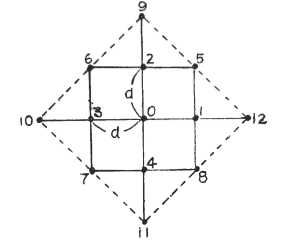
\includegraphics[scale=0.45]{./imgs/wiki/12-points-fd.png}
    \caption{computation domain and grid system}     
    \label{fig:1}
\end{figure*}
The law of conservation of energy is verified.
\begin{equation}
    J(A, B) = 2J_1(A, B)-J2(A, B)
\end{equation}
\begin{equation}
    J_1(A, B) = \frac{1}{3}[J^{++}(A, B)+J^{+\times}(A, B)+J^{\times+}(A, B)]
\end{equation}
\begin{equation}
    J^{++}(A, B) = \frac{1}{4d^2}[(A_1-A_3)(B_3-B_4)-(A_2-A_4)(B_1-B_3)]
\end{equation}
\begin{equation}
    J^{+\times}(A, B)= \frac{1}{4d^2}[A_5(B_2-B_1)-A_7(B_3-B_4)+A_6(B_3-B_2)-A_8(B_4-B_1)]
\end{equation}
\begin{equation}
    J^{\times+}(A, B) = \frac{1}{4d^2}[A_1(B_5-B_8)-A_3(B_6-B_7)-A_2(B_5-B_6)+A_4(B_8-B_7)]
\end{equation}

\begin{equation}
    J_2(A, B) = \frac{1}{3}[J^{\times\times}(A, B)+J^{\times+}(A, B)+J^{+\times}(A, B)]
\end{equation}
\begin{equation}
    J^{\times\times}(A, B) = \frac{1}{8d^2}[(A_5-A_7)(B_6-B_8)-(A_6-A_8)(B_5-B_7)]
\end{equation}
\begin{equation}
    J^{+\times}(A, B)= \frac{1}{8d^2}[A_5(B_9-B_{12})-A_7(B_{10}-B_4)-A_6(B_9-B_{10})+A_8(B_{12}-B_{11})]
\end{equation}
\begin{equation}
    J^{\times+}(A, B) = \frac{1}{8d^2}[A_9(B_6-B_5)-A_{11}(B_7-B_8)+A_{10}(B_7-B_6)-A_{12}(B_8-B_5)]
\end{equation}
Here $A_i, B_i (i=1,......12)$ is the corresponding value of A, B at $i$-th points.
\section{3D model}
As for the 3D model, the motion equations are,
\begin{equation}
    \begin{cases}
        \frac{du}{dt}=\frac{uv\tan\phi}{r}-\frac{uw}{r}-\frac{1}{\rho}\frac{\partial p}{r\cos\phi\partial\lambda}+fv-\hat{f}\omega+F_{\lambda}\frac{d}{dt}+\frac{u^2}{\tan\phi}{r} \\
        \frac{dv}{dt}=-\frac{u^2\tan\phi}{r}-\frac{vw}{r}-\frac{1}{\rho}\frac{\partial p}{r\partial \phi}-fu+F_{\phi} \\    
        \frac{d\omega}{dt}=\frac{u^2+v^2}{r}-\frac{1}{\rho}\frac{\partial p}{\partial r}-g+\hat{f}u+F_r\\
    \end{cases}
\end{equation}
\subsection{sigma vertial coordinate}
A vertical coordinate for atmospheric models defined as pressure normalized by its surface value, or as the difference in pressure and its value at the top
of the model atmosphere normalized by the surface value of this difference. \newline
Thus,
\begin{equation}
    \sigma=\frac{p-p_T}{p_S-p_T}
\end{equation}

\begin{figure*}
    \centering
    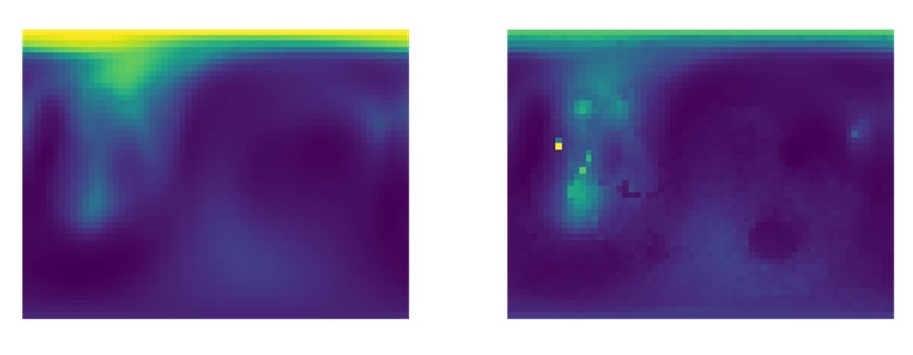
\includegraphics[scale=0.45]{./imgs/wiki/sigma_diff.JPG}
    \caption{Before sigma and sigma}     
    \label{fig:2}
\end{figure*}
The difference could be seen in figure 2.
\subsection{Hybrid sigma}
The hybrid $\sigma$ coordinate remodified the high pressure level. 
\begin{equation}
    p_d=B(\eta)(p_s-p_t)+[\eta-B(\eta)](p_0-p_t)+p_t
\end{equation}
where $p_0$ is a reference sea-level pressure. Here, $B(\eta)$ defines the relative weighting between the terrain-coordinate for $B(\eta)=\eta$ and
reverts to a hydrostatic pressure coordinate for $B(\eta)=0$. To smoothly transition from a sigma near the surface to a pressure coordinate at upper levels,
$B(\eta)$ is defined by a third order polynomial \newline
\begin{equation}
    B(\eta)=c_1+c_2\eta+c_3\eta^{2}+c_4\eta^{3}
\end{equation}
By applying the boundary conditions, there should be,
\begin{equation}
    \begin{cases}
        B(1)=1\\
        B_{\eta}=1\\
        B(\eta_c)=0\\
        B_{\eta}(\eta_c)=0\\
    \end{cases}
\end{equation}
such that,
\begin{equation}
    \begin{cases}
        c_1=\frac{2\eta_c^2}{(1-\eta_c)^3}\\
        c_2=\frac{-\eta_c(4+\eta_c+\eta_c^2)}{(1-\eta_c)^3}\\
        c_3=\frac{2\eta_c(1+\eta_c+\eta_c^2)}{(1-\eta_c)^3}\\
        c_4=\frac{-(1+\eta_c)}{(1-\eta_c)^3}\\        
    \end{cases}
\end{equation}
where $\eta_c$ is a specified value of $\eta$ at which it becomes a pure pressure coordinate.
The difference could be seen in figure 3.
\begin{figure*}
    \centering
    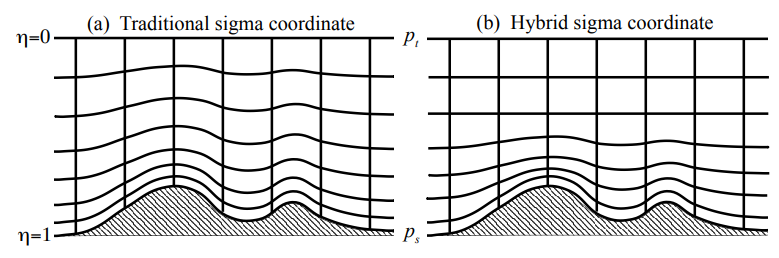
\includegraphics[scale=0.45]{./imgs/wiki/hybridsigma.png}
    \caption{sigma and hybrid sigma}     
    \label{fig:3}
\end{figure*}
What should the $\eta_c$ be for Mars?
\end{document}